\documentclass[12pt]{article}
\renewcommand{\baselinestretch}{1.5}
\usepackage{epsf,epic,eepic,eepicemu}
%\documentstyle[epsf,epic,eepic,eepicemu]{article}
\usepackage[utf8]{inputenc}
\usepackage[czech]{babel}     
\usepackage{ae}
\usepackage{fancyhdr}

\usepackage[a4paper]{geometry} 
\geometry{top=3.5cm, bottom=3.5cm, left=3.5cm, right=2.5cm}

\usepackage[dvipdfm]{graphicx}
\author{Martin Venuš, Jaroslav Líbal}

\graphicspath{{img/}}

\usepackage[dvipdfm,unicode,colorlinks]{hyperref}
\hypersetup{bookmarksopen=false,hypertexnames=false, anchorcolor=black, citecolor=black, filecolor=black, linkcolor=black, menucolor=black, urlcolor=blue, pdfauthor={Martin Venuš, Jaroslav Líbal}, pdftitle={Dokumentace - semestrální projekt MI-VMW}}

\begin{document}
%\oddsidemargin=-5mm \evensidemargin=-5mm \marginparwidth=.08in
%\marginparsep=.01in \marginparpush=5pt \topmargin=-15mm
%\headheight=12pt \headsep=25pt \footheight=12pt \footskip=30pt
%\textheight=25cm \textwidth=17cm \columnsep=2mm \columnseprule=1pt
%\parindent=15pt\parskip=2pt

% ============================ Hlavička dokumentu ==================================================================
\begin{center}
\bf Semestrální projekt MI-VMW 2010/2011\\[5mm]
    Flickr - feature-based reranking\\[5mm]
       Jaroslav Líbal\\
       Martin Venuš\\[5mm]
FIT ČVUT\\[2mm]
magisterské studium\\[2mm]
Kolejní 550/2, 160 00 Praha 6\\[2mm]
7. prosince 2010
\end{center}

%\pagestyle{empty} %get rid of header/footer for toc page
\newpage
\tableofcontents
\newpage
%\pagestyle{fancy}

\section{Zadání úlohy}
%Jarda
Cílem úlohy je naprogramovat aplikaci, která nejprve pomocí Flickr API vyhledá obrázky na základě klíčového slova a tyto obrázky následně přeřadí na základě analýzy barev obsažených v~obrázku. Aplikaci je možné psát v~libovolném programovacím jazyce, ale prostředkem pro vizualizaci výsledků vyhledávání musí být webový prohlížeč.

Pro realizaci naší úlohy jsme zvolili programovací jazyk PHP a framework Nette.

Aplikace poběží na adrese \url{http://vmw.wsolution.cz/}


\section{Definice základních barev}
%Jarda
Pro určování jednotlivých barev v~obrázku bylo nejprve nutné nadefinovat seznam základních barev na které se následně identifikují barvy rozpoznané v~obrázku. Při sestavování tohoto seznamu jsme použili standardní \texttt{Web safe} barvy, kterých je 216. Ke každé z~nich jsme poté přiřadili jednu z~námi stanoveného seznamu jedenácti barev které nejblíže odpovídá a ze kterých může uživatel při zadávání dotazu vybírat.

\section{Získání dat z~Flickr API}
%Martin
Pro získání obrázků z~Flickr API využíváme třídu \texttt{phpFlickr}\footnote{\url{http://www.phpflickr.com/}}, která využívá REST API Flickeru. Pro získání fotografií využíváme metodu \texttt{flickr.photos.search} s~následujícími argumenty:
\begin{itemize}
\item \texttt{tags} - klíčová slova
\item \texttt{tag\_mode} = any (klíčová slova oddělená čárkou jsou vyhledávána v~režimu OR)
\item \texttt{sort} = relevance (řazení výsledku podle relevance)
\item \texttt{media} = photos (chceme pouze fotografie)
\item \texttt{per\_page} - počet požadovaných fotografií\footnote{Flickr API vrací v~některých případech fotografie v~nedostatečném rozlišení. Takové fotografie nelze použít pro barevnou analýzu a nejsou tak zobrazovány ve výsledcích vyhledávání. Je tedy možné, že při zadání požadavku na vyhledání 20 fotografií bude výsledek obsahovat méně fotografií.}
\end{itemize}

Metoda, která zajišťuje zaslání požadavku na Flickr API vrací pole výsledků. V~dalším kroku ověřujeme, zda jsou všechny fotografie v~dostatečném rozlišení (tedy, zda existuje fotografie označená jako \texttt{Large}) - ke každé fotografii získáme podrobné informace o~dostupných rozlišeních pomocí metody \texttt{flickr.photos.getSizes}. Fotografie, které nejsou k~dispozici v~rozlišení označeném jako \texttt{Large} vyřadíme.

V~dalším kroku podrobujeme fotografie analýze barev.

\section{Analýza barev v~obrázku}
%Martin
Pro získání dominantní barvy obrázku využíváme metodu Bena Hindmarcha z~roku 2007 (26. 6. 2007). Metoda rozdělí obrázek na zadaný počet bloků a v~těchto blocích pak vyhledává dominantní barvu. Metoda vrací dominantní barvu každého bloku obrázku.

Abychom byli schopni určit základní barvu je pak nutné porovnat získané barvy jednotlivých bloků s~barvami uloženými v~databázi a uložit si příslušnou základní barvu. Nalezení nejbližší barvy probíhá pomocí výpočtu vzdálenosti od jednotlivých barev uložených v~databázi tak, že porovnáme součet kvadrátů jednotlivých barevných složek získané barvy bloku v~obrázku s~barvou uloženou v~databázi. V~databázi je 216 barev a pro každou barvu je uvedena základní barva.

Následně pole obsahující počet jednotlivých základních barev vyskytujících se v~obrázku a na konci metody vypočteme procentní podíl hledané barvy, který vracíme jako návratovou hodnotu metody.

\section{Hodnocení}
Pro hodnocení algoritmus jsme zvolili náhodný obrázek v~rozlišení 1024x768 pixelů, ve kterém vyhledáváme černou barvu. 
%Martin
\renewcommand{\figurename}{Graf}
\setcounter{figure}{0}
\begin{figure}[ht]
\centering       
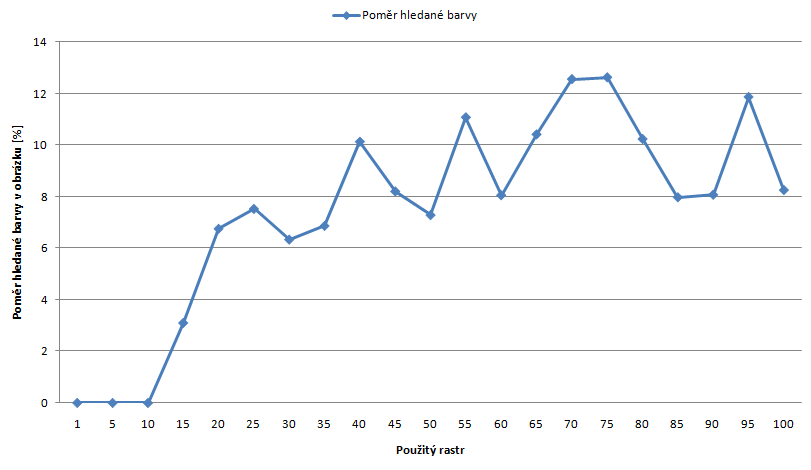
\includegraphics[scale=0.6]{graf.png}
\caption{Poměr hledané barvy v~obrázku v~závislosti na použitém rastru.}
\label{graf}
\end{figure}

Z~grafu je zřejmé, že při zvolení příliš nízké hodnoty rastru ($< 20$) jsou získané hodnoty příliš zkreslené. To je způsobeno tím, že je obrázek rozdělen na příliš málo částí. Při zvolení rastru $\geq 20$ jsou již získané hodnoty dobré a zvyšování hodnoty rastru nepřináší výraznější zlepšení. 

Použijeme-li získané hodnoty pro hodnotu rastru $\geq 20$ získáme následující statistické ukazatele:
\begin{itemize}
\item Počet hodnot: 17
\item Minimum: 10,13
\item Maximum: 8,25
\item Aritmetický průměr: 9,07
\item Medián: 6,75
\item Rozptyl: 4,05
\item Směrodatná odchylka: 2,01
\end{itemize}

\section{Závěr}
%Jarda
Práce na semestrálním projektu byla zajímavá a podařilo se nám splnit všechny body zadání. Vyzkoušeli jsme si možnosti implementace Flickr API, které pro nás však bylo poměrně zklamáním. Rychlost odpovědí API na zasílané požadavky je velice špatná a prakticky tak znemožňuje jeho reálné využití.

\end{document}
